% A short report (named PE report xxx.pdf) that describes the most im-
% portant programming info (such as the main data structure and the basic
% 5content of the three functions). Time measurements of the PageRank iterations
% function, when varying the number of OpenMP threads, should be pre-
% sented as well as the information of the compiler and hardware used.
% Programming issues relevant for performance optimization (if any) should
% also be included. IN4200 students should also provide a short discus-
% sion about the maximumly achievable (ideal) computing speed of the
% PageRank iterations function

% TODO: Produce timing graphs
% Which graphs:
% Time usage on different number of threads oon pagerank
% Time usage of readfile and topwebpages

\documentclass[10pt, a4paper]{amsart}
%\usepackage[english,norsk]{babel}
\usepackage[english]{babel}
\usepackage[utf8]{inputenc}

\usepackage{geometry}   % Margins
\usepackage{graphicx}   % Images
\usepackage{float}      % Image floating
\usepackage{siunitx}    % SI-units
\usepackage{amsmath}
\usepackage[boxed]{algorithm2e}
\usepackage{verbatim}
\usepackage{url}
\usepackage{hyperref}
\usepackage{listings}
\usepackage{framed}
\numberwithin{figure}{section}
\numberwithin{table}{section}
\bibliographystyle{plain}

\usepackage{color}
%\usepackage{multicol}
%\setlength\columnsep{14pt}

\definecolor{codegreen}{RGB}{0, 146, 146}
\definecolor{codegray}{rgb}{0.4,0.4,0.4}
\definecolor{codeblue}{RGB}{0, 109, 219}
\definecolor{backcolour}{rgb}{0.9,0.9,0.9}

\lstdefinestyle{mystyle}{
    backgroundcolor=\color{backcolour},
    commentstyle=\color{codegreen},
    keywordstyle=\color{magenta},
    numberstyle=\tiny\color{codegray},
    stringstyle=\color{codeblue},
    basicstyle=\footnotesize,
    breakatwhitespace=false,
    showstringspaces=false,
    breaklines=true,
    captionpos=b,
    keepspaces=true,
    numbers=left,
    numbersep=5pt,
    showspaces=false,
    basicstyle=\footnotesize \ttfamily \color{black} \bfseries,
    xleftmargin=0.4cm,
    frame=tlbr, framesep=0.1cm, framerule=0pt,
    showtabs=false,
    tabsize=2
}

\lstset{style=mystyle}


\title[Computing PageRank]{IN3200 - Partial exam \\ \large
Computing PageRank}
\author[Candidate no. 15229]{Candidate no. 15229 \\ \\ \today}


\begin{document}

\maketitle

%\begin{center}
%    Source code can be found in GitHub repository at \url{https://github.com/ejhusom/IN3200/IN3200_PE_ejhusom}
%\end{center}

\tableofcontents

%\begin{multicols}{2}
\section{Introduction}

The goal of this project was to implement the PageRank algorithm, which is a part of Google's search engine. Input is taken from a file containing a \textit{web graph}, which has information about all the links (\textit{edges}) between a set of webpages (\textit{nodes}). This web graph is then used to calculate a score for each page, which indicate the importance of the page based on how many and which webpages that are linked to it, either by outbound or inbound links.

The main focus of the project was to produce effective code, partly by parallelizing the PageRank algorithm using OpenMP, which is an application programming interface for shared memory multiprocessing programming. I tested the code on three large web graphs from the Stanford Large Network Dataset Collection\cite{stanford}, which are called \textit{web-NotreDame}, \textit{web-Stanford} and \textit{web-BerkStan}. The last of these web graphs is the largest one, with 685,230 nodes and 7,600,595 edges, and with such a large amount of data that needs to be processed there is also need for highly effective code.

This report contains information about how the program works, and an analysis of the time usage for different parameters and number of parallel threads.


\section{Program structure}

\subsection{Functions}
In this section I will explain the basic content of the code. The source code is split into two files. The file called \texttt{PE\_main\_15229.c} contains the \texttt{main} function, that sets up the necessary arrays and variables and calles the functions that compute the PageRank score. This file also contains code to measure time usage for all the functions. Info about compilation and execution is found in the README-file of the project.

The file called \texttt{PE\_functions\_15229.c} contains in total five functions, and the details of these are explained below. Some of the algorithms and loops are somewhat hard to explain in consice terms, but comments are also provided in the source code.

\subsubsection{\texttt{read\_graph\_from\_file()}}
This function's task is to read all the data from a file, and then set up a \textit{hyperlink matrix} based on the data. The matrix is of size $N \times N$, where $N$ is the number of webpages in the data set, and the matrix elements are defined as
\begin{equation}
    a_{ij} =
    \begin{cases}
            \frac{1}{L(j)}, &         \text{if there's an inbound link from webpage no. \textit{j}, } (i\neq j),\\
            0, &         \text{otherwise}.
    \end{cases}
\end{equation}
where $L(j)$ is the number of outbound links from webpage no. $j$. Self-linkage should not affect the PageRank score, so any links from a webpage to itself is removed. This results in a sparse matrix, where most elements are zero, and we use the Compressed Row Storage (CRS) format to store this matrix. This format consist of the following arrays:
\begin{itemize}
    \item \texttt{val}: Contains the non-zero values of the matrix.
    \item \texttt{col\_idx}: Contains the column index of the corresponding element of \texttt{val}.
    \item \texttt{row\_ptr}: Contains the index where a new row starts in the array \texttt{val}.
\end{itemize}

This function starts with reading in the number of nodes and edges in the web graph, which is used to allocate arrays of the correct size. An example of the accepted format of the web graph is as follows:
\begin{verbatim}
# Directed graph (each unordered pair of nodes is saved once): 8-webpages.txt
# Just an example
# Nodes: 4 Edges: 7
# FromNodeId    ToNodeId
0       1
0       2
1       3
2       3
2       1
3       1
3       2

\end{verbatim}
All the edges/links in the file are then read through, with an if-test to remove potential self-links. At the same time the program counts how many outbound and inbound links each node has. This can then be used to find \texttt{row\_ptr}, since the inbound link count corresponds to how many values there are in each row in the matrix. The array \texttt{row\_ptr} is then found  by summing up this element count for each row.

Another necessary part of the PageRank algorithm (explained below) is to find any dangling webpages, that is webpages with no outbound links. This is simply done by examining the outbound link count, and see which page indices that has noe outbound links.

The most complex part of this function is finding the elements of \texttt{col\_idx}. We cannot assume that the edges in the web graph are sorted in any way, so either we have to sort the data, or we have to use an algorithm that does not depend on sorting (or only minimally depend on sorting). Sorting arrays up to sizes of 7 million elements (in the case of the \textit{web-BerkStan} data set) can be relatively expensive, and therefore we want to avoid that. The algorithm I came up with iterates through the edges as they are presented in the web graph, and because we already have produced the array \texttt{row\_ptr}, we know the minimum and maximum index of where a column number is to be placed in \texttt{col\_idx} based on what row number it has. In this loop the values of \texttt{col\_idx} will be placed in the correct domain (i.e. the correct row), but not necessarily in the correct order within that domain. This is then solved by sorting the column indeces within each domain. This algorithm is not easily explained in just a few lines, but may become clearer when looking directly at the source code and following the data flow. The minimal use of sorting ensures that even the hyperlink matrix of the \textit{web-BerkStan} data set is set up in a few seconds (see accurate timing information in the next section).

The last step is finding \texttt{val}, which is easily done by using the outbound link count for each column.

In this function I have included some comment sections that are marked with \texttt{DEBUG}, where it is possible to get printouts of certain arrays. This is done to make debugging easy by checking the values that are produced by the code.

\subsubsection{\texttt{PageRank\_iterations()}}
The goal of this function is to produce a vector $\mathbf{x}$ containing the PageRank scores of all the webpages. And initial guess
\begin{equation}
    \mathbf{x}^0 = \frac{1}{N}\begin{bmatrix}1 \\ 1 \\ \vdots \\ 1\end{bmatrix}
\end{equation}
is used, $N$ being the number of webpages, and then the following formula is used:
\begin{equation}
    \mathbf{x}^k = \frac{(1 - d + d \cdot W^{k-1})}{N}\begin{bmatrix}1 \\ 1 \\ \vdots \\ 1\end{bmatrix} + d \cdot \mathbf{A}\mathbf{x}^{k-1},
    \label{eq:pagerank}
\end{equation}
where $\mathbf{A}$ is the hyperlink matrix and $d$ is a damping constant that usually is set to 0.85. $W^{k-1}$ is the sum of the PageRank scores, from the previous iteration, of all the dangling webpages. Equation \ref{eq:pagerank} is iterated through until the scores converge. The stopping criterion I used in my code is
\begin{equation}
    \sum_{j=1}^{N} \left( |x_j^k - x_j^{k-1}| \right) < \epsilon,
\end{equation}
where $\epsilon$ is a given threshold. The default threshold value in my code is set to \SI{1e-10}, because the difference between converged PageRank scores usually is of magnitude \SI{1e-4} (see example of results in the next section). With this convergence threshold the results should be of good enough numerical precision. The reason for choosing to sum up the differences between all elements from on iteration to the next, is that it is a simpler implentation (with minimal if-tests) compared to finding the maximum difference of all the elements in the array.

The PageRank equation is implented inside a while-loop that checks the stopping criterion for each iteration. In order to maximize the efficiency of this function I have also used OpenMP to parallelize the code. Number of threads has to be given as a command line argument. Loops with few iterations are not worth parallelizing, because OpenMP overhead leads to bad performance. There are usually several ways to parallelize a certain code block, and I chose to use a rather straight-forward method, by calling \texttt{\#pragma omp parallel for} on the matrix-vector-multiplication (MVM) in the PageRank algorithm (and also when intializing the result vector). This lets OpenMP divide the labour automatically on the number of threads that has been assigned. The function also counts the number of iterations that are needed for the result to converge within the given threshold.


\subsubsection{\texttt{top\_n\_webpages()}}
This function takes (among other things) a number $n$ as input argument, and provides a list of the $n$ highest ranked webpages, together with their PageRank scores and their indeces. It is of course possible to do this by sorting the complete array of PageRank scores from highest to lowest, and then printing out the first $n$ of those, but considering that the number $n$ typically will be much smaller than the number of webpages (which for our test data sets was several hundred thousand), it is almost always unnecessary to sort the whole array. Therefore I wanted to avoid having to sort the large array of scores, because this is relatively expensive in terms of processing power. Instead, the function takes a copy of the PageRank score array, iterates through the array and finds the highest score, prints out the rank, index and score of that page, and then sets that element to zero. The algorithm is set up as follows:

\begin{algorithm}[H]
\SetAlgoLined
n = number of top webpages to print\;
max = 0\;
\For{n webpages}{
  \For{all elements in PageRank score array}{
  \If{element is bigger than max}{
  set max to value of element\;
  store index of element\;
  }
   }
   print the page index and score of the maximum element\;
   set maximum element to zero\;
   reset max to zero\;
 }
\end{algorithm}

This is a quick and easy way of making sure that in the next iteration, the algorithm will find the second highest score, and at the same time avoiding potential problems with multiple pages having the same score (this is usually only a problem for very small data sets).

\subsubsection{\texttt{sort()} and \texttt{swap()}}
A part of the method used to set up the CRS matrix depended on a sorting algorithm, which consists of the functions \texttt{sort()} and \texttt{swap()}. These two functions were taken from the first exercise set of the subject IN3200 at the University of Oslo\cite{exercises}.


\section{Results and time measurements}
In this section I will present time measurements with different parameters. The hardware used is the following:
\begin{itemize}
  \item Processor: Intel Core M-5Y71 CPU @ 1.20GHz $\times$ 4
  \item Memory: 8 GB DDR3L SDRAM @ 1600 MHz - PC3L-12800
\end{itemize}
The program was run on Ubuntu 18.04 with the C compiler \texttt{gcc}, version 7.3.0.

To better understand the performance differences, I have listed the size of the data sets in table \ref{tab:datasets}.

\begin{table}
    \caption{Size of the data sets used in this project.}
    \label{tab:datasets}
    \begin{tabular}{lll}
        Data set & Number of nodes & Number of edges \\
        \hline
        \textit{web-NotreDame} & 325,729 & 1,497,134 \\
        \textit{web-Stanford} & 281,903 & 2,312,497\\
        \textit{web-BerkStan} & 685,230 & 7,600,595\\
    \end{tabular}
\end{table}

\subsection{Time measurements of parallelized function}
The time measurements for the function \texttt{PageRank\_iterations()} are shown in figure \ref{fig:timing_parallel} for all three data sets. The data sets are processed with varying number of threads for the parallelized part of the code, and each execution is run 5 times to obtain an average. In the graph, all measurements are plotted to give an impression of the spread of the data, and the mean is plotted with a line and a cross. The difference is most notable with the \textit{web-BerkStan} dataset, and the precise mean run time for this dataset are also presented in table \ref{tab:timing_parallel}.

For all the datasets, the most drastic improvement happens when going from 1 to 2 threads. For \textit{web-BerkStan} and \textit{web-Stanford}, the run time actually increases when going from 2 to 3 threads, and the same happens for \textit{web-NotreDame} when going from 3 to 4 threads. It is possible that the performance is decreased by heat generation in the CPU, since the measurements were obtained by executing the program several consecutive times. Each test was only done 5 times, which also means that it could be coincidential that the run times happened to be slightly slower for a larger number of threads, even though one would expect at least some performance gain when increasing the thread number. Lastly, it is also possible that my implementation of the parallelized code, and the use of OpenMP, was not done in an optimal way. I chose a rather simple way to use OpenMP, and it is of course a possibility that mistakes in the source code leads to suboptimal performance.

In any case, we can see that for the largest data set, \textit{web-BerkStan}, there is a clear trend of higher performance when increasing the number of threads. The run time is almost cut in half when going from 1 to 4 threads.

\begin{table}[H]
    \caption{Mean time measurements for the function \texttt{PageRank\_iterations()} on the \textit{web-BerkStan} dataset, with different number of threads. Measurements are averaged over 5 runs per thread number.}
    \label{tab:timing_parallel}
    \begin{tabular}{ll}
        Number of threads & Mean run time [s] \\
        \hline
        1 & 8.4848562 \\
        2 & 5.0602186 \\
        3 & 5.1053918 \\
        4 & 4.4328932 \\
    \end{tabular}
\end{table}

\begin{figure}
    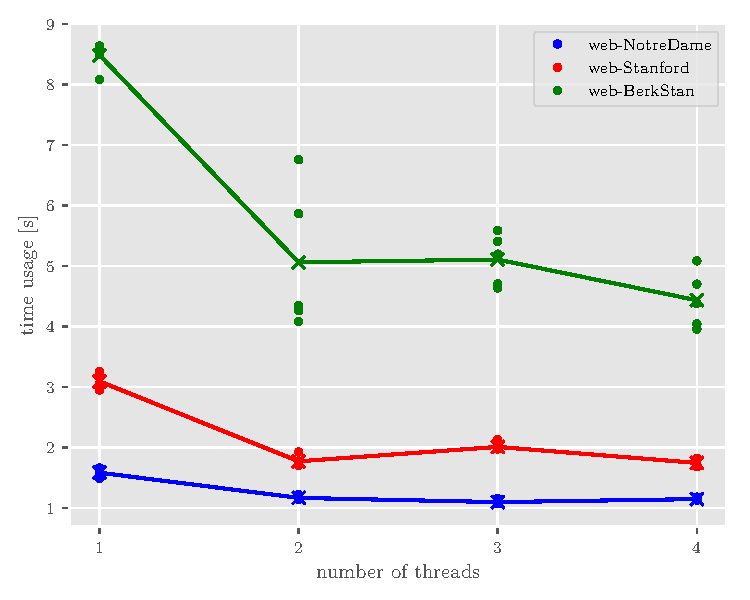
\includegraphics{../runtime.pdf}
    \caption{Run time for the three different data sets, for different number of threads. Measurements are represented as dots, and the mean as crosses with line.}
    \label{fig:timing_parallel}
\end{figure}

\subsection{Time measurements of serial functions}
The time measurements results for the functions \texttt{read\_file\_from\_graph()} and \texttt{top\_n\_webpages()} are presented in table \ref{tab:timing_serial}. As we can see, the run times are pretty similar for \textit{web-NotreDame} and \textit{web-Stanford}. The former has a larger number of nodes, but the latter has a larger number of edges. The function \texttt{top\_n\_webpages()} iterates through an array that has one element per node in the data set, which means that this function should use longer time for the \textit{web-NotreDame} data set, and this is indeed the case. The processing time of the function \texttt{read\_file\_from\_graph()} depends more on the number of edges, which also explains why the run time is longer for the \textit{web-Stanford} data set. The last data set, \textit{web-BerkStan}, has a significantly larger amount of both edges and nodes, and therefore has the longest processing time for these two functions.

\begin{table}[H]
    \caption{Time measurements for the two serial functions for three different data sets. The measurements are averaged over 5 runs per function per data set.}
    \label{tab:timing_serial}
    \begin{tabular}{lll}
        Data set & Run time \texttt{read\_file\_from\_graph()} [s] & Run time \texttt{top\_n\_webpages()} [s] \\
        \hline
        \textit{web-NotreDame} & 0.40107 & 0.0081102 \\
        \textit{web-Stanford} & 0.67739 & 0.0069156\\
        \textit{web-BerkStan} & 3.15396 & 0.0212098\\
    \end{tabular}
\end{table}


\subsection{Results of \texttt{top\_n\_webpages()}}

For easy comparison with other programs, I have provided the results from my source code on the \textit{web-NotreDame} data set, executed with the default parameters, in table \ref{tab:notredame_results}.

\begin{table}[H]
    \caption{The 8 webpages with the highest calculated PageRank score, using the source code in this project on the \textit{web-NotreDame} data set.}
    \label{tab:notredame_results}
    \begin{tabular}{lll}
        Rank & Page index & PageRank score \\
        \hline
        1. & 1963 & 0.0056267674\\
        2. & 0 & 0.0054045118\\
        3. & 124802 & 0.0033262290\\
        4. & 12129 & 0.0028570560\\
        5. & 191267 & 0.0027487313\\
        6. & 32830 & 0.0027318341\\
        7. & 3451 & 0.0025899846\\
        8. & 83606 & 0.0024596915\\
    \end{tabular}
\end{table}

\bibliographystyle{unsrt}
\bibliography{references}


%\end{multicols}
\end{document}
